% xv2-acmsmall-sample.tex, dated March 6 2012
% This is a sample file for ACM small trim journals
%
% Compilation using 'acmsmall.cls' - version 1.3 (March 2012), Aptara Inc.
% (c) 2010 Association for Computing Machinery (ACM)
%
% Questions/Suggestions/Feedback should be addressed to => "acmtexsupport@aptaracorp.com".
% Users can also go through the FAQs available on the journal's submission webpage.
%
% Steps to compile: latex, bibtex, latex latex
%
% For tracking purposes => this is v1.3 - March 2012

\documentclass[prodmode,acmtecs]{acmsmall} % Aptara syntax


% Package to generate and customize Algorithm as per ACM style
\usepackage[ruled]{algorithm2e}
\renewcommand{\algorithmcfname}{ALGORITHM}
\SetAlFnt{\small}
\SetAlCapFnt{\small}
\SetAlCapNameFnt{\small}
\SetAlCapHSkip{0pt}
\IncMargin{-\parindent}

% Metadata Information
% \acmVolume{9}
% \acmNumber{4}
% \acmArticle{39}
% \acmYear{2010}
% \acmMonth{3}

% Copyright
%\setcopyright{acmcopyright}
%\setcopyright{acmlicensed}
%\setcopyright{rightsretained}
%\setcopyright{usgov}
%\setcopyright{usgovmixed}
%\setcopyright{cagov}
%\setcopyright{cagovmixed}

% DOI
% \doi{0000001.0000001}

%ISSN
% \issn{1234-56789}

% Document starts
\begin{document}

% Page heads
\markboth{Y. Xie et al.}{Ranking Code Completion Candidates}

% Title portion
\title{Ranking Code Completion Candidates}
\author{Yanan Xie
\affil{yaxie@ucsc.edu}
Yifei Wu
\affil{ywu151@ucsc.edu}
Ziyi Chen
\affil{zchen139@ucsc.edu}
}
\begin{abstract}
Code completion is becoming a basic feature to all kinds of IDEs. It helps programmers to avoid typos and learn new languages fast. With the development of hardware performance and machine learning techniques, a lot of work could be done to further improve the code completion performance. Traditional code completion function lists all reserved words and variable names that match user’s input and then rank those matches in alphabetical order. We propose a new code completion candidate ranking method which aims at ranking those candidates with contextual syntax and semantic information. A code completion plugin is also built for Sublime Text - a very popular cross-platform code editor.
\end{abstract}


\maketitle


\section{Introduction}

Code completion (also known as content assist) is now one of most used features in modern integrated development environments(IDEs)\cite{murphy2006java}. There are many mainly three reasons for its popularity. First, typos can be very common when we try to type lengthy words without the help of code completion. Second, the more complex a project is, the more method names, variable names and class names we need to memorize. Code completion can help developers to narrow down possible proposals to a limited subset and speed up coding. Third, with a strong code completion system, developers are more likely to adopt informative words or short phrases naming methods, variables and classes. Those more descriptive names usually result in more readable and undestandable code\cite{bruch2009learning}. 

Recent researches focused on ranking member method candidates, since we can expect dozens of member methods in a class. Those proposed methods are either learning from exisiting examples\cite{bruch2009learning,raychev2014code} or from past code history\cite{robbes2008program}. 

As shown in Fig. \ref{fig:xcode}, modern IDE like Xcode still have a lot of space to improve. 

\begin{figure}
\centerline{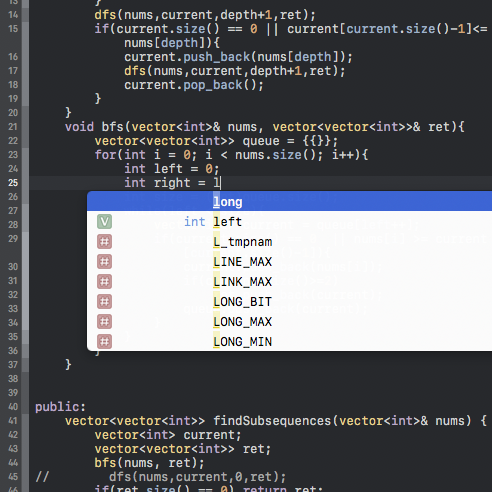
\includegraphics[width=1.0\textwidth]{xcode}}
\caption{Screenshot on Xcode}
\label{fig:xcode}
\end{figure}


In this project, we build a C language code completion plugin for Sublime Text where we mainly address two tasks. The first one is to determine which reserved word (e.g., {\it if}, {\it for}, {\it while}) or what kind of category (i.e., variable name, declaration) is more likely to be enter next. The second part is to rank variables in the context.



\section{Generating Abstract Syntax Tree}
Clang is a C based language front-end for the LLVM compiler\cite{lattner2004llvm}. The main reason we choose clang over gcc is that clang generates neater AST(Abstract Syntax Tree) than gcc does. Fig. \ref{fig:ast example} shows an AST segment generated by clang. 

\section{Ranking variables}
In this section, we talk about how to rank variables. According our experience, recently modified(assigned) or declared variables are more likely to be used. So we evaluate the relation of the distance between declaration/assignment and reference of variables, in order to rank previous variables at a certain point according to the distance. \\
We download git source code from github, which is written by c language, as our training data. Then we use Clang to generate AST of all those c files. Clang is a compiler front-end which is faster and neater that gcc. An example of ast is Fig. \ref{fig:ast example}. The front part is all "TypedefDecl", which is the ast structure of head file. But we only need to find out all declaration and assignment operation in cpp file. Since variables are only effective in certain function, we first find out all functions by "FunctionDecl" and then look out corresponding variables. The declaration statement is shown as "DeclStmt" as well as the function parameter "ParmVarDecl". The assignment statement consists of "BinaryOperator" with "=" and "UnaryOperator", which is "++" or "--". Use function name and variable name as key, ast line number and variable numbers as value to generate a dictionary. Then match all "DeclRefExpr" to find out usage of variables and use former dictionary to find distance of most recently declaration and modification. The result is shown below;

                                                           



\section{Modeling syntax}
In this section, we will try to figure out the relation between different types. At the beginning, we deal with the AST files we get from the previous section. 

An example of AST is shown in Fig. \ref{fig:ast example}. The first token(ForStmt, DeclStmt, VarDel, IntegerLiteral) in each line is the type in AST. After learning the source codes of git\cite{torvalds2010git}, we get more than 70 kinds of different types. However, code completion aims to complete English word only. In other words, we only deal with type names, variable names, function names and reserved words. Thus, we should simplify these kinds of types. 

Here are our rules of simplification:

If a token contains “Decl”, we sort it to declaration, which is the format of “type-name + variable names”. If a token contains “Expr”, we sort it to expression, which begins with “variable names”. If a token contains “Stmt”, we remain it as reserved word, such as “ForStmt” is “for”, “WhileStmt” is “while”. If a toke not contains “Decl”, “Expr”, “Stmt”, we sort it to else and ignore it in the following process.

After simplification, we get 22 kinds of types. In order to rank the candidates, we use a simple statistical model - hidden Markov model which assumes the distribution of next token is only determined by current token\cite{rabiner1986introduction}. Then we calculate order-relations in all AST files. We calculate two kinds of relations. One is A$\longrightarrow$B. Another is A$\longrightarrow$B$\longrightarrow$C. Using these statistics results. We can get the possibility of all types when we know the previous code. 

Table \ref{tab:SyntaxOne} is part of statistics result of A$\longrightarrow$B and Table \ref{tab:SyntaxTwo} is part of statistics result of A$\longrightarrow$B$\longrightarrow$C. From this we can see that with privous two tokens we can get a more accurate token.


\begin{figure}
\centerline{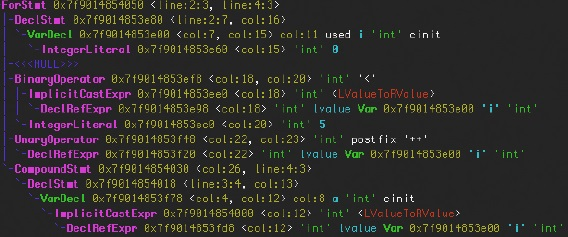
\includegraphics[width=0.9\textwidth]{ast_example.jpg}}
\caption{An AST segment generated by clang}
\label{fig:ast example}
\end{figure}


\begin{table}%
\tbl{Partial Relation A$\longrightarrow$B\label{tab:SyntaxOne}}{%
\begin{tabular}{|l|l|l|l|}
\hline
Condition	 &Top Candidate	 &2nd Candidate	 &3rd Candidate\\\hline
FunctionDecl &	Declaration	 &FunctionDecl	 &ReturnStmt\\\hline
Declaration	 &Declaration &	FunctionDecl	 &Variable\\\hline
ReturnStmt	 &Variable	 &IfStmt	 &ForStmt\\\hline
Variable	 &Variable &	ReturnStmt	 &IfStmt\\\hline
IfStmt &	Variable	 &- &	-\\\hline
WhileStmt &	Variable &	-	 &-\\\hline
ForStmt	 &Declaration	 &Variable	 &IfStmt\\\hline
ContinueStmt	 &IfStmt	 &Variable	 &CaseStmt\\\hline
\end{tabular}}
\end{table}%


\begin{table}%
\tbl{Partial Relation A$\longrightarrow$B$\longrightarrow$C\label{tab:SyntaxTwo}}{%
\begin{tabular}{|l|l|l|l|}
\hline
Condition A&Condition B	 &Top Candidate	 &2nd Candidate\\\hline
empty &	FunctionDecl	 &Declaration	 &-\\\hline
FunctionDecl	 &Declaration &	Declaration	 &FunctionDecl\\\hline
Declaration	 &Declaration	 &Declaration	 &ForStmt\\\hline
Declaration	 &ReturnStmt &	Variable	 &-\\\hline
Declaration &	Variable	 &Variable &	-\\\hline
Declaration &	IfStmt &	Variable	 &-\\\hline
\end{tabular}}
\end{table}%




\section{Hacking the editor}

Sublime Text is a sophisticated text editor for code, markup and prose\cite{skinner2016sublime}. The reason we choose Sublime Text as the software we build the plugin for is that it is one of most popular cross platform code editors. 

In order to provide suggestions to the editor, we need to write a function named {\it on\_query\_completions} which returns all the suggestions in an array. Since it is an synchronized method, it is not supposed to run a while. It should return the result imediatelly. So we should analyze the user code in another method called {\it on\_modified\_async} which runs asynchronously after user change the code. With those two methods in a Python program, we can analyze user code and provide our suggestions through Sublime Text. Fig. \ref{fig:sublimeplugin} shows a screenshot on our plugin.

\begin{figure}
\centerline{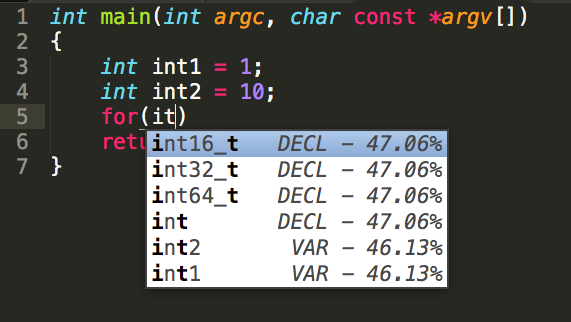
\includegraphics[width=1.0\textwidth]{sublimeplugin}}
\caption{Screenshot on the plugin}
\label{fig:sublimeplugin}
\end{figure}


% Bibliography
\bibliographystyle{ACM-Reference-Format-Journals}
\bibliography{acmsmall-sample-bibfile}
 


\end{document}
% End of v2-acmsmall-sample.tex (March 2012) - Gerry Murray, ACM


